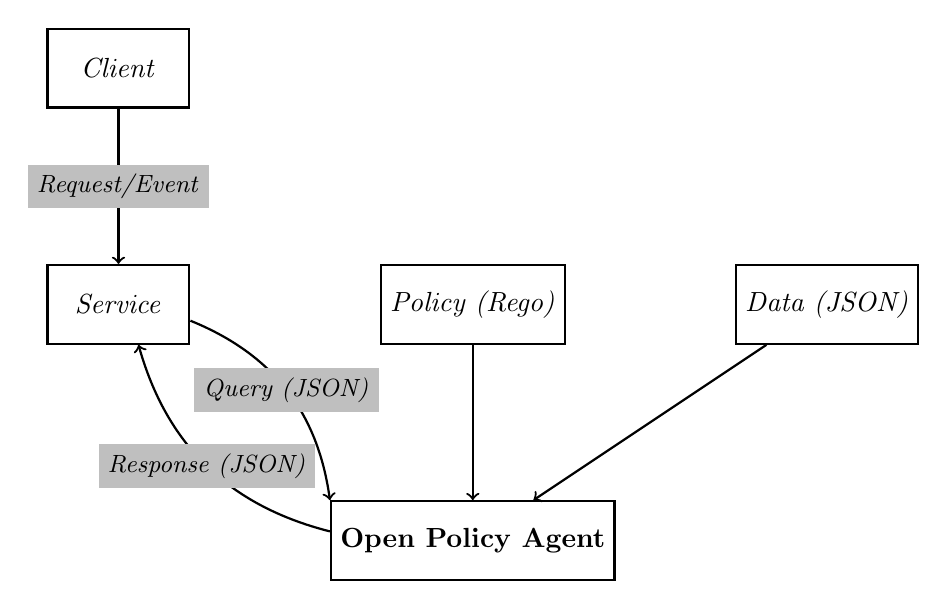
\begin{tikzpicture}[
        s/.style={draw,thick,rectangle,minimum height=10mm, minimum width=18mm},
        e/.style={fill=gray!50},
        xsh/.style={xshift=15mm}
    ]

    \tikzset{
        node distance=30mm,
    }

    \node[s] (client) {\textit{Client}};
    \node[s,below of=client] (service) {\textit{Service}};
    \node[s,right of=service,xsh] (policy) {\textit{Policy (Rego)}};
    \node[s,right of=policy,xsh] (data) {\textit{Data (JSON)}};
    \node[s,below of=policy] (OPA) {\textbf{Open Policy Agent}};

    \draw[->,thick]
        (client) edge node[e] {\small \textit{Request/Event}} (service)
        (service) edge[bend left] node[e] {\small \textit{Query (JSON)}} (OPA.north west)
        (OPA) edge[bend left] node[e] {\small \textit{Response (JSON)}} (service)
        (policy) edge (OPA)
        (data) edge (OPA)
        ;
    
\end{tikzpicture}
